%*********************************************************************************************
% Written By: Carson McAfee 
% Written on 23/07/2015

% This is a generic tex document written for use in SANSA documentation.
% Read the comments for guidance regarding the changes/options that can be done.

% This is a generic report document for use by a SANSA person.
% It has a number of options:
% -> Select if the first page is numbered.
% -> Select if every page is numbered, or just the Title Page.
%
% If the document is large enough for a TOC, then rather use the Month End Report Template.
% This is more suited for that need.
%*********************************************************************************************
%*********************************************************************************************
\documentclass[a4paper,12pt]{article}
\usepackage[pdftex]{graphicx}
\usepackage[]{cite}
\usepackage{longtable}
\usepackage[a4paper,left=25mm,right=25mm,top=25mm,bottom=45mm]{geometry}
\usepackage{fancyhdr, graphicx}

%*********************************************************************************************
%*********************************************************************************************
% This is where I will place custom commands.

\newcommand*{\TitleFont}{%
      \usefont{\encodingdefault}{\rmdefault}{b}{n}%
      \fontsize{46}{35}%
      \selectfont
}

\fancypagestyle{fancyheader}{
    \fancyhead[R]{\scriptsize University of the Witwatersrand\\ Faculty of Engineering and the Built Environment \\  School of Electrical and Information Engineering}
    \fancyhead[L]{
\includegraphics[width=1.5cm]{Images/EIE_logo.jpg}}
    \fancyfoot[C]{} 

}

\fancypagestyle{fancyplain}{
    \fancyhead[R]{\scriptsize University of the Witwatersrand\\ Faculty of Engineering and the Built Environment \\  School of Electrical and Information Engineering}
    \fancyhead[L]{
\includegraphics[width=1.5cm]{Images/EIE_logo.jpg}}
    \fancyfoot[C]{\thepage} 
}
%*********************************************************************************************
%*********************************************************************************************
%This is where the content of the Title Page gets added.
% Minor adjustments will be necessary for a specific user, and never again.

%This is where you select if you want all the pages to have the SANSA logo.
\pagestyle{fancyplain}
%\pagestyle{plain}

\begin{document}
\setcounter{page}{0} %Uncomment this if you want start counting from first page. Adjust page syles.
\vspace{2cm}
\title{ Wits University VLF Station - Handover Installation Notes }
\date{23/07/2015}
\author{Carson McAfee - 303033}
\maketitle
\thispagestyle{fancyheader}

%*********************************************************************************************
%*********************************************************************************************
% This is where you start adding content to the document. Enjoy.

\section{Network/MAC Address}
At the time of installation there was an issue with the servers, so the Wandboard mac could not be added to the servers, and therefore could not get a IP address.\\
\\
As a work around I did a mac spoof from a PC that I had previously registered. The original PC was part of my Weather Sat project. \\
\\
The Weather Sat Mac address was: 	02:8f:05:02:4e:2e\\
The WandBoard Quad Mac address is: 	00:1f:7b:b4:11:1c\\
\\
SO to do the mac spoofing I wrote a script to be run by root at startup. The script is called tempMacSpoof, and is located in /home/ubuntu/. I have deliberately put it here to embarrass future managers into sorting out the problem correctly.\\
\\
The script is as follows:
\begin{verbatim}
#!/bin/sh
ip link set dev eth0 address 02:8f:05:02:4e:2e
\end{verbatim}

To run the script I added the following line to roots crontab:
\begin{verbatim}
@reboot /home/ubuntu/tempMacSpoof
\end{verbatim}

Now the mac address will be spoofed automatically on boot. Always. \textbf{BUT THIS IS A TEMP SOLUTION AND MUST BE CHANGED. ASK NIXON.}

\subsection{SSH Access}
To access the wandboard you can SSH in. The ip address is ``146.141.116.190''. User name and password is: ``ubuntu''.

\begin{verbatim}
ssh ubuntu@146.141.116.190
\end{verbatim}



\section{Startup Scripts}

I have a feeling that there will be a number of startup scripts at the end of the project. They will each be discussed separately. Hopefully a summary of the scripts will be placed here in a later document.

\subsection{Main System Startup}
This is an all in one script written by Jason Smit in 2015. It is located in \emph{/startscript.sh} (IE absolute root).

\begin{itemize}
 	\item Creates a record of restarts. This is so that you can know how many times the system has gone down. Which is important when working with a Solar Based system.
 	\item It mounts the external HDD. Im not entirely sure if I like this, but it does have its merits. I normally prefer it to be in the fstab, but his has the benefit of mounting any new drive (useful for when a drive is removed and replaced with a new one). BUT!!! You must make sure that the drive FS type is correct. Jasons test drive was a ext4 type, and the new drives are NTFS. I have changed that in the script.
 	\item The script then configures the recording software, and also prepares log files. I like this.
 \end{itemize} 

 The last item is of most importance. The software Jason has used is called ``vlftools'' from http://abelian.org/vlfrx-tools/. He uses this software to configure the sound card, record a stream, and write the stream to a current file type (saved in a folder with a naming convention).\\
 \\
 He also has a number of useful log files:
 \begin{itemize}
 	\item /var/log/record/downtime.log 	: This keeps track of the downtime events.
 	\item /var/log/record/start.log 	: This keeps a record of whether the system starts correctly.
 	\item /var/log/record/vtcard.log 	: Log of vttools config info.
 \end{itemize}

 \subsection{Wav File Creator}
  The next file of interest is also located in the root directory (``/''). \textbf{Im not sure if i like having them here. I think they should be kept in a scripts folder under the main users account.}\\
  \\
  This script starts on startup. Im not actually sure where this script or the main script are being called. They should be in a crontab given the repeatable nature, but they aren't in roots or ubuntu's user crontabs. Strange.\\
  \\
  Anyway this script converts the VTtools audio buffer into wav files and stores them in /mnt/drive/wav . The naming convention is self explanatory.

\section{Data Analysis}
So on startup everything will start automatically. Give it at least 2 minutes to adjust before checking. It begins by recording audio and saving it into an vttools buffer in /mnt/drive/. Then the buffer is converted into a .wav file and saved in /mnt/drive/wav/. So this is where you can look for the most recent recordings. But then what...\\
\\
Well I would prefer to have as little processing done on the wand board as possible. So you need to copy the audio files from the wandboard to your local machine:
\begin{verbatim}
	scp /mnt/drive/wav/150723*.wav username@youripaddress:/path/on/your/system/
\end{verbatim}

Once you have a local copy of the data you can listen to it, or you can produce spectrograms to visually inspect the data.\\
\\
I have included two scripts that can be used ``Spectrogram.py'' and ``group\_spec\_report.py''. The first script is meant for individual file checking:

\begin{verbatim}
	./Spectrogram.py -sd 150723-101800Wvlf1.wav 
\end{verbatim}

This will produce two png images for the North-South and East-West channels. The ``-sd'' is for save and display and can be used individually. 

\begin{figure}[h!]
	\centering
	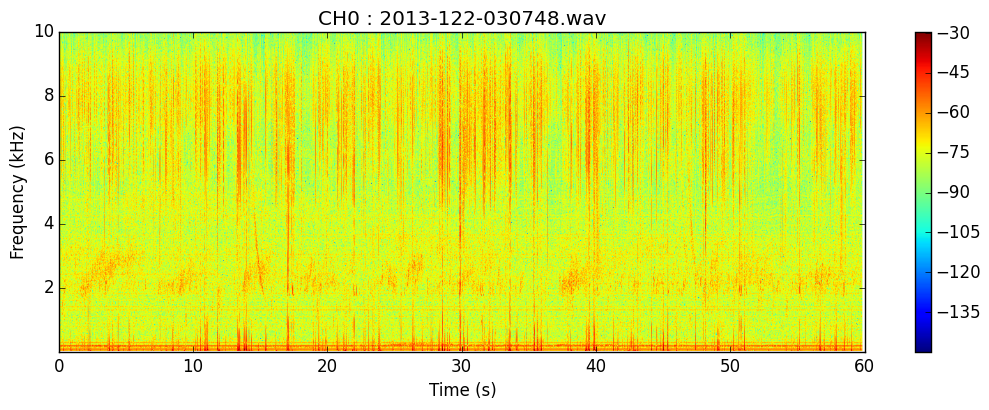
\includegraphics[width=15cm]{Images/MarionCH0.png}
	\caption{Marion Island CH0}
	\label{fig:MARIONCH0}
\end{figure}

\begin{figure}[h!]
	\centering
	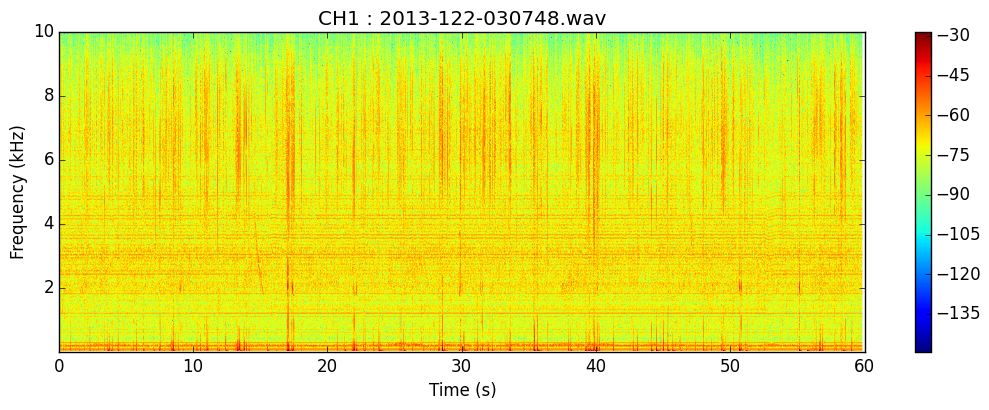
\includegraphics[width=15cm]{Images/MarionCH1.png}
	\caption{Marion Island CH1}
	\label{fig:MARIONCH1}
\end{figure}

\begin{figure}[h!]
	\centering
	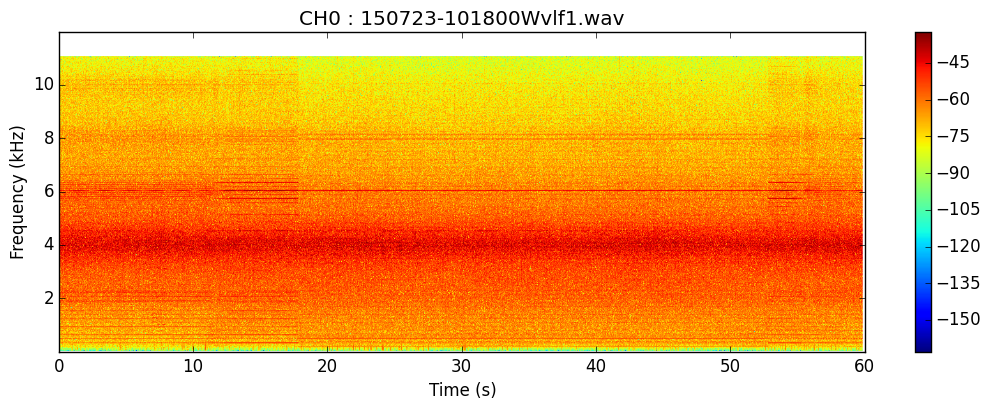
\includegraphics[width=15cm]{Images/WitsCH0.png}
	\caption{Wits University CH0}
	\label{fig:WITSCH0}
\end{figure}

\begin{figure}[h!]
	\centering
	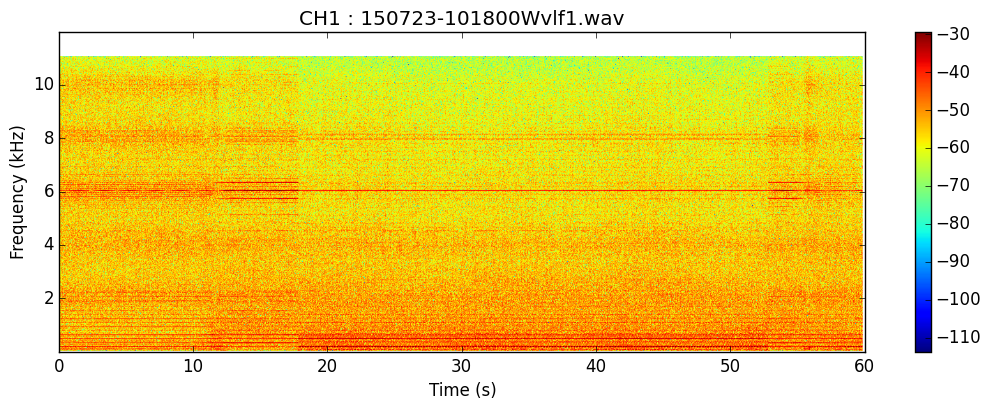
\includegraphics[width=15cm]{Images/WitsCH1.png}
	\caption{Wits University CH1}
	\label{fig:WITSCH1}
\end{figure}
\newpage

Figures \ref{fig:MARIONCH0} and \ref{fig:MARIONCH1} show a spectrogram from Marion Island. This is what we need to aim to achieve. The Wits signal is shown in Figures \ref{fig:WITSCH0} and \ref{fig:WITSCH1}. The wits signal is way too noisy at the moment.\\
\\
The second file compiles a range of .wav files into a single PDF of spectrograms.

\begin{verbatim}
	./group_spec_report.py 150723*.wav 
\end{verbatim}

These scripts are fairly basic, and can be changed if needed. The colour of the spectrograms can be changed. The original setting was ``binary'' which is black and white and is often easier to differentiate signals.\\
\\
These scripts should run fairly easily. You need to install matplotlib and numpy. Remember that everything is python2 and not python3! The only difficulty is Scikits Audiolab. With Audiolab there were no install files from the official repositories. I have included the files in this folder, and they can be installed as follows:

\begin{verbatim}
tar -xvf scikits.audiolab-0.11.0.tar.gz
cd scikits.audiolab-0.11.0/
sudo python setup.py install
\end{verbatim}


\newpage
\section{TO DO LIST}
Unfortunately  have run out of time on this project. I hope that when I hand it over it will be in a state of recording VLF data. But there is still a lot to do with it, and I hope that there is someone to do it.\\
\\
I think Jason Smit will be keen to get involved further, and I think that he may be a good choice. Anyway here is a list of things that need to be done:

\begin{itemize}
	\item GPS Timing System.
	\item Fibre-Ethernet installation Box.
	\item VLF Website.
	\item Fix the Record timing.
	\item Baudline.
	\item Daily Data Management.
	\item Check Gain Switch.
	\item User Account Settings.
	\item Find correct spelling of spectrograms.
	\item Figure out which channel is which...
	\item General Gain Situation.
\end{itemize}

\subsection{GPS Timing System}
This is very very important. For WWLLN to add us we will need to have a very accurate time resolution. At the moment the wandboard sources its time from a online NTP server. This is ok for standard applications but for a TOA location system the time is not accurate enough.\\
\\
We have 2 GPS units for the project, and they are quite easy to use. Basically we need to setup a local NTP server on the wandboard that sources its time from the GPS. This is easy. The hard bit is going to be the Pulse Per Second (PPS) setup. Unfortunately the serial port on the wandboard is not a true serial port, but rather a USRT converter. Sneeky bastards! On a normal serial port the PPS can be sourced directly. However we will now need to use the wandboards GPIO pins to source the PPS. I am not sure how tricky this will be. But in theory it shouldn't be that hard. The PPS is supplied by the GPS unit, and it is literally a Pulse Per Second. The ideal is that the pulse is measured (ie the input pin goes high), an interrupt happens, and a file is written to or an event is triggered. This trigger is then fed to the GPS software and is used to keep an accurate time. Mitchel Cox has offered to help with advice on this matter, and how to integrate the PPS with the GPIO pins. \\
\\
Other than that, the only thing left to do is make the wiring harness, and the GPIO harness. The power can be provided by the USB micro port or maybe directly from the Power supply board.\\
\\
The main source of info on GPS software is from here:\\
http://www.catb.org/gpsd/gpsd-time-service-howto.html\\
http://www.catb.org/gpsd/installation.html\\
\\
This is a software reference with lots of info on setting up linux software, and creating a NTP server. Remember that the main time source should come from the GPS and not the network Make sure that this is the case.\\
\\
Other sources of interest are:\\
http://www.lammertbies.nl/comm/info/GPS-time.html\\
http://www.rfdesign.co.za/Files/5645456/PDF/NEO\_7N\_SMART\_PS.pdf\\
http://www.gpskit.nl/connections-en.htm\\
http://gpsppssync.sourceforge.net/\\
\\
Setting up the GPS and software should take 30 min. Getting the PPS working is the real challenge.

\subsection{Fibre-Ethernet installation Box}

In the back corner of the Aircon room I have placed the fibre to Ethernet converter on a table. This is a bit expose, and should be put in a nice box and mounted to the wall of nearby beam. Warning notices need to be placed on the box, at the power point, and where the fibre cable comes out the wall.

\subsection{VLF Website}

This is a project that I feel is necessary once the system is working. It can be very impressive.\\
\\
I would like to create a website for the VLF/Space Weather data. This ideal has been taken from the SANSA setup. The SANSA setup is called a ``Dashboard''. Basically it is a webpage showing live data. Basically new spectrograms are uploaded to the webpage constantly. In addition to this we could feed live data on power and energy usage of the system. WWLLN data. Temperature data. Automatic Whistler detector count (from VTtools). Solar flare data from a Russian website. PC operational stats. And maybe some other interesting stats. \\
\\
The end goal would be to do what SANSA did. Basically we get a big 42 inch screen and mount it in a public space. Then we attach a raspberry pi to the screen to display the Space Weather data. The reason for the big screen is to show all the data on one page. This has a number of benefits. It raises awareness of the project, creates interest in the project, helps identify problems quickly, and its really cool.\\
\\
Creating something like this is quite easy. Basic web page hosted by the school servers, a few basic scripts run from crontab, and we are set to go. In addition to this we could create a project wiki on the same website, and list all the projects that will be done, or have been done by the school on VLF. Think of it like the VLF research group web page.

\subsection{Fix the Record timing}
I am not convinced by the VTtools software. The ``/Startupscript.sh'' script starts VTtools recording at 20000 Hz, and continuously in 1 min segments. However I found that when processing the audio files the Frequency band shows 11 kHz, which would suggest that the true sampling frequency is 22 kHz. Also the file does not seem to be a full 60 seconds. I had to change both spectrogram scripts to only process the first 59.8 seconds (``stop = 59.8 * r.samplerate''). Please find out what is actually happening.

\subsection{Baudline}

An additional tool that may be worth looking into is ``Baudline''. This is a real time spectrum measurement tool so that you can see the state of the VLF spectrum in real time. Useful for fault finding as well as a number of other applications. To use it you will have to investigate setting up a ``jackd'' server, to split the line in input and pass one stream over the network for clients to monitor.

\subsection{Daily Data Management}

Looking in ``/mnt/drive/wav'' you will see that there are a lot of files. These need to be managed correctly. I would suggest creating a storage folder on the HDD, and then running a daily crontab (at 3:00 AM every day) to move the days data to the folder and then gzip the files to save on space. Should be easy to do.

\subsection{Check Gain Switch}

I noticed that there is an issue with the splitter board rotator switch. For reference, when looking at the top of the switch turn the dial counter clockwise all the way. This is the zero input setting. One turn clockwise will supply 1\% of the input voltage to the filter circuit. One more turn to the right will select 10\% of the input voltage. One last turn to the right will select 100\% of the input voltage.\\
\\
I noticed that all the gain settings are too high. This is clear by the spectrograms, as well as the fact that the overvoltage LED's on the board are continuously on. These should only come on occasionally when there is a particularly big spheric.\\
\\
The main concern here is that the LED's turn off on the 10\% setting. This should not happen, and I think there is a problem with the 50 ohm resistors being used, or maybe the soldering underneath.

\subsection{User Account Settings}

I don't like the fact that we are using the standard Ubuntu user name for the user account. I would like to create a user called ``Wits\_VLF'', or something of the sort. More professional in my opinion. I would also like the password to be made unique. Soon the WWLLN guys will need external access, which will mean that the wand board will be susceptible to external attach, so the security of the system and our network needs to be considered.\\
\\
Once the new user has been created, I would like the old user to be deleted. The next step would be to remove the script responsibilities from the sudo user to our user. I feel this is better practice. Root user should not be in charge of our measurement system and data. A private user such as ourselves should have standard system permissions. So basically migrate the operational scripts to the new user.

\subsection{Figure out which channel is which}

This is fairly important. Systematically check which channel (0 or 1) is related to the North-South or East-West antennas. Then mark the boxes and cct boards. Then update this document with that information.

\subsection{General Gain Situation}

This is the most important item. It is clear that there is a problem with the system. By inspecting the splitter board it is clear that the overvoltage LED's are on on every setting, which means that the voltage is too high, and is saturating the line in. The LED's should ideally be off continuously, and only flash occasionally when there is a big spheric.\\
\\
So I have narrowed down a few possibilities. First, on the preamp board I have set the first stage gain to have a 150 times gain, rather than the original 100 times gain. Change the 15 kohm resistor to a 10 kohm one and see if that helps. There is however a good chanced that my preamp board is kak. Testing it was quite hard given the high gain, so it is hard to say how well it s actually working. Also I removed a DC cap filter from the inputs, which may have been a bad idea, but helped clean the signal during my testing. So basically look at the board again, and try make it better. Ultimately its whole purpose is simply a gain stage. The splitter is responsible for the filtering.\\
\\
It may be a getter idea to redesign the board (hopefully what the 4th years will be doing). It may also be a good idea to try a transistor first stage gain, I was just a bit scared of the design for it.\\
\\
Mitchel Cox also gave a good suggestion. He reckons that the input impedance of the opamps (OPA847) should be ridiculously high, and we could try connect the antennas directly to the inputs. Therefore skip the transformers. Not a bad idea.\\
\\
Another consideration is that the alsa settings or sound card config is wrong. Also check that the VT config is correct. The current ISO image was developed on the single core wand board. The one in use is the quad core. I loaded the same card in both, but there may be some differences. Jason Smit should be able to help in this regard.\\
\\
But basically the first aim is to drop the gain level so that the LED's go off. It may be a good idea to use a variable gain stage on an op amp, but be careful where this is done, and what is used. I used a trim pot on the first stage op amp feedback loop. This was a bad idea because the frequency was distorted. However using a carbon pad swivel pot may act better. Once you can tune the gain a bit, I am sure that the signal will be better.

\end{document}
